\documentclass[a4paper, twocolumn, superscriptaddress,prl]{revtex4}  %% REVTeX 4.0
\usepackage{graphicx}
\usepackage{amsmath,amssymb,braket}

\begin{document}
\title{Enhancing resolution in fluorescence microscopy by second order coherence}
\author{Clayton Seitz}
\affiliation{Department of Physics, Indiana University, Indianapolis}

\begin{abstract}
Optical fluctuation microscopy has become a popular tool in fluorescence microscopy, yet background photons degrade signal correlations and reduced resolution. Here, we describe the scaling of second order coherence with the signal to background ratio and describe implications for optical fluctuation imaging. 
\end{abstract}

\maketitle 

Superresolution optical fluctuation imaging (SOFI) is a simple, versatile microscopy method popular for biological imaging. It provides the possibilities of enhancement beyond the diffraction limit for both lateral and axial resolution, reduction of influence of background illumination, technical simplicity, and possibility to use rather low intensities of the field. It is suitable for superresolution three-dimensional (3D) imaging of living cells and subcellular structures. SOFI can be combined with other microscopy methods, such as light-sheet fluorescence microscopy and image scanning microscopy, and is easily integrated into existing microscopic setups: for example, wide-field, confocal, and total internal reflection fluorescence microscopy. SOFI functions by measuring high-order intensity correlations of randomly emitting fluorescent sources. Initially, SOFI was demonstrated with blinking quantum dots (QDs). Soon, it was applied using organic dyes, fluorescent proteins, and semiconducting polymer dots. Later, SOFI was shown to work by speckled illumination with fluorophores without natural blinking.


\subsection{Basic Scheme}

We consider a set of $N$ point sources in the object plane labeled by continuous valued coordinates $r=(x,y)$ and labeled in the image plane $s=(u,v)$.  respectively. The field is then treated by a simplified model consisting of a single mode (Vlasenko 2020). The positive frequency field operator in the object plane reads

\begin{equation}
E_{0}^{+}(r) \sim \sum_{i=1}^{N}\delta(r-r_{i})a_{j}
\end{equation}

The continuous field in image space is then 

\begin{equation*}
E^{+}(s) =  \int d^2 r E_{0}^{+}(r) O(s-r)
\end{equation*}

We take the point spread function $O$ to be isotropic Gaussian. Since our detectors must be discrete, the total field at a pixel $\tilde{E}^{+}(s_{n})$ in image space is then given by integrating over pixels

\begin{align*}
\tilde{E}^{+}(s_{n}) &=  \int d^2 s E^{+}(s) \\
&=  \int d^2 s \int d^2 r E_{0}^{+}(r) O(s_n-r)\\
&=  \int d^2 r E_{0}^{+}(r) \int d^2 s \; O(s_n-r)
\end{align*}

where $\int d^2 s \; O(s_n-r) = \frac{1}{2}\lambda_{x} \lambda_{y}$ and, for example,

\begin{align*}
\lambda_{x} = \mathrm{erf}\left(\frac{u_n+\frac{1}{2}-x_i}{\sqrt{2}\sigma}\right) -\mathrm{erf}\left(\frac{u_n-\frac{1}{2}-x_i}{\sqrt{2}\sigma}\right)
\end{align*}


Combining this result with (1), we see the above integral is simply a sum of terms of the form

\begin{align*}
\tilde{E}^{+}(s_{n}) &=  \frac{a_{i}}{2}\lambda_{x}(u_n) \lambda_{y}(v_n)
\end{align*}

\onecolumngrid

\begin{figure}[h] 
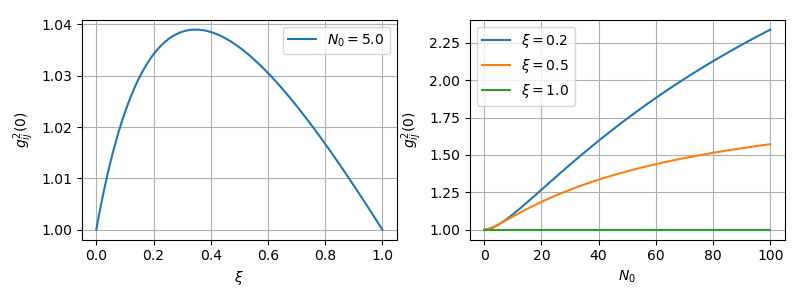
\includegraphics[width=16cm]{Figure_1.png}
\end{figure}    
\twocolumngrid

\subsection{Zero-lag order coherence for an isolated emitter}

Photoswitching fluorescent emitters are described by the density matrices

\begin{equation*}
\rho_{S} = \sum_{k}\xi_{k}\ket{\alpha_k}\bra{\alpha_k}\;\;\rho_{B} = \ket{\beta}\bra{\beta}
\end{equation*}

We consider an isolated fluorescent emitter in the presence of a coherent background signal. The emitter can access a discrete set of states $\ket{\alpha_k}$, with occupancy probabilities $\xi_{k}$ and amplitude $\alpha_k$  $\langle n\rangle = \bra{\alpha_{k}} n\ket{\alpha_{k}} = \lvert\alpha_{k}^{2}\rvert$. We consider only zero-lag coherence, therefore neglecting the temporal structure of the jump process. For an isolated emitter, we have

\begin{equation}
\tilde{E}^{+}(s_{n}) =  \hat{a}\Lambda + \hat{b}
\end{equation}

where $\Lambda = \frac{1}{2}\lambda_{x}(u_n) \lambda_{y}(v_n)$. The non-normalized second order coherence in the image plane reads 

\begin{align*}
G^{2}_{nm}(0) &= \langle \tilde{E}^{-}(s_n)\tilde{E}^{-}(s_m)\tilde{E}^{+}(s_n)\tilde{E}^{+}(s_m)  \rangle\\
&= \Lambda_{n}^{2}\Lambda_{m}^{2}\sum_{k}\xi_{k}\mu_{k}^2 + \mu_{B}(\Lambda_{n}^{2} + \Lambda_{m}^{2})\sum_{k}\xi_{k}\mu_{k} + \mu_{B}^2
\end{align*}

which in the normalized form reads

\begin{align*}
g^{2}_{nm}(0) &= G^{2}_{nm}(0) / \langle I_{n}\rangle \langle I_{m}\rangle
\end{align*}

where the intensity expectation at a detector element is of course $\langle I_{n}\rangle = \Lambda_{n}^{2}\sum_{k}\xi_{k}\mu_{k} + \mu_{B}$. For example, if we have a two-level system consisting of a fluorescent state with amplitude $\alpha$ and the vacuum state, this becomes

\begin{equation*}
g^{(2)}_{ij}(0) = \frac{\xi\lvert\alpha\rvert^{4}}{\xi^{2}\lvert\alpha\rvert^{4}} = \frac{1}{\xi}
\end{equation*}

As $\xi\rightarrow 1$ (always on) we recover a coherent state. As $\xi\rightarrow 0$ we observe $g^{(2)}_{ij}(0) > 1$ i.e., bunching.


\begin{thebibliography}{31}
\expandafter\ifx\csname natexlab\endcsname\relax\def\natexlab#1{#1}\fi
\expandafter\ifx\csname bibnamefont\endcsname\relax
  \def\bibnamefont#1{#1}\fi
\expandafter\ifx\csname bibfnamefont\endcsname\relax
  \def\bibfnamefont#1{#1}\fi
\expandafter\ifx\csname citenamefont\endcsname\relax
  \def\citenamefont#1{#1}\fi
\expandafter\ifx\csname url\endcsname\relax
  \def\url#1{\texttt{#1}}\fi
\expandafter\ifx\csname urlprefix\endcsname\relax\def\urlprefix{URL }\fi
\providecommand{\bibinfo}[2]{#2} \providecommand{\eprint}[2][]{\url{#2}}

\bibitem[{\citenamefont{Fujita et~al.}(2007)}]{KawataPRL07}
\bibinfo{author}{\bibfnamefont{K.}~\bibnamefont{Fujita}} \bibnamefont{et~al.},
  \bibinfo{journal}{Phys. Rev. Lett.} \textbf{\bibinfo{volume}{99}},
  \bibinfo{eid}{228105} (\bibinfo{year}{2007}).

\bibitem[{\citenamefont{{Gustafsson}}(2005)}]{Gustafsson_SSI_PNAS05}
\bibinfo{author}{\bibfnamefont{M.~G.~L.} \bibnamefont{{Gustafsson}}},
  \bibinfo{journal}{Proc. Nat. Acad. Sci.} \textbf{\bibinfo{volume}{102}},
  \bibinfo{pages}{13081} (\bibinfo{year}{2005}).

\bibitem[{\citenamefont{Hell and Wichmann}(1994)}]{STED_Hell_OL1994}
\bibinfo{author}{\bibfnamefont{S.}~\bibnamefont{Hell}} \bibnamefont{and}
  \bibinfo{author}{\bibfnamefont{J.}~\bibnamefont{Wichmann}},
  \bibinfo{journal}{Optics Letters} \textbf{\bibinfo{volume}{19}},
  \bibinfo{pages}{780} (\bibinfo{year}{1994}).

\bibitem[{\citenamefont{Betzig et~al.}(2006)}]{PALM_Betzig_Science2006}
\bibinfo{author}{\bibfnamefont{E.}~\bibnamefont{Betzig}} \bibnamefont{et~al.},
  \bibinfo{journal}{Science} \textbf{\bibinfo{volume}{313}},
  \bibinfo{pages}{1642} (\bibinfo{year}{2006}).

\bibitem[{\citenamefont{Hess et~al.}(2006)\citenamefont{Hess, Girirajan, and
  Mason}}]{PALM_Sam_Hess_BiophysJ2006}
\bibinfo{author}{\bibfnamefont{S.}~\bibnamefont{Hess}},
  \bibinfo{author}{\bibfnamefont{T.}~\bibnamefont{Girirajan}},
  \bibnamefont{and} \bibinfo{author}{\bibfnamefont{M.}~\bibnamefont{Mason}},
  \bibinfo{journal}{Biophysical journal} \textbf{\bibinfo{volume}{91}},
  \bibinfo{pages}{4258} (\bibinfo{year}{2006}).

\bibitem[{\citenamefont{Michael J.~Rust and Zhuang}(2006)}]{STORM_NatMet06}
\bibinfo{author}{\bibfnamefont{M.~B.} \bibnamefont{Michael J.~Rust}}
  \bibnamefont{and} \bibinfo{author}{\bibfnamefont{X.}~\bibnamefont{Zhuang}},
  \bibinfo{journal}{Nature Methods} \textbf{\bibinfo{volume}{3}},
  \bibinfo{pages}{793} (\bibinfo{year}{2006}).

\bibitem[{\citenamefont{Dertinger et~al.}(2009)}]{SOFI_DertingerPNAS2009}
\bibinfo{author}{\bibfnamefont{T.}~\bibnamefont{Dertinger}}
  \bibnamefont{et~al.}, \bibinfo{journal}{Proc. Nat. Acad. Sci.}
  \textbf{\bibinfo{volume}{106}}, \bibinfo{pages}{22287}
  (\bibinfo{year}{2009}).

\bibitem[{\citenamefont{Lidke
  et~al.}(2005)}]{Localization_by_blinking_Heintzmann_OpEx2005}
\bibinfo{author}{\bibfnamefont{K.}~\bibnamefont{Lidke}} \bibnamefont{et~al.},
  \bibinfo{journal}{Optics Express} \textbf{\bibinfo{volume}{13}},
  \bibinfo{pages}{7052} (\bibinfo{year}{2005}).

\bibitem[{\citenamefont{Giovannetti et~al.}(2004)\citenamefont{Giovannetti,
  Lloyd, and Maccone}}]{Quantum_Enhanced_measurements_Science2004}
\bibinfo{author}{\bibfnamefont{V.}~\bibnamefont{Giovannetti}},
  \bibinfo{author}{\bibfnamefont{S.}~\bibnamefont{Lloyd}}, \bibnamefont{and}
  \bibinfo{author}{\bibfnamefont{L.}~\bibnamefont{Maccone}},
  \bibinfo{journal}{Science} \textbf{\bibinfo{volume}{306}},
  \bibinfo{pages}{1330} (\bibinfo{year}{2004}).

\bibitem[{\citenamefont{Brida et~al.}(2010)\citenamefont{Brida, Genovese, and
  Berchera}}]{Sub_shot_noise_imaging_NatPhot2010}
\bibinfo{author}{\bibfnamefont{G.}~\bibnamefont{Brida}},
  \bibinfo{author}{\bibfnamefont{M.}~\bibnamefont{Genovese}}, \bibnamefont{and}
  \bibinfo{author}{\bibfnamefont{I.}~\bibnamefont{Berchera}},
  \bibinfo{journal}{Nature Photonics} \textbf{\bibinfo{volume}{4}},
  \bibinfo{pages}{227} (\bibinfo{year}{2010}).

\bibitem[{\citenamefont{D'Angelo et~al.}(2001)\citenamefont{D'Angelo, Chekhova,
  and Shih}}]{Lithography_proof_of_principle_PRL2001}
\bibinfo{author}{\bibfnamefont{M.}~\bibnamefont{D'Angelo}},
  \bibinfo{author}{\bibfnamefont{M.~V.} \bibnamefont{Chekhova}},
  \bibnamefont{and} \bibinfo{author}{\bibfnamefont{Y.}~\bibnamefont{Shih}},
  \bibinfo{journal}{Phys. Rev. Lett.} \textbf{\bibinfo{volume}{87}},
  \bibinfo{pages}{013602} (\bibinfo{year}{2001}).

\bibitem[{\citenamefont{Afek et~al.}(2010)\citenamefont{Afek, Ambar, and
  Silberberg}}]{Afek_Science2010}
\bibinfo{author}{\bibfnamefont{I.}~\bibnamefont{Afek}},
  \bibinfo{author}{\bibfnamefont{O.}~\bibnamefont{Ambar}}, \bibnamefont{and}
  \bibinfo{author}{\bibfnamefont{Y.}~\bibnamefont{Silberberg}},
  \bibinfo{journal}{Science} \textbf{\bibinfo{volume}{328}},
  \bibinfo{pages}{879} (\bibinfo{year}{2010}).

\bibitem[{\citenamefont{Walther
  et~al.}(2004)}]{Four_photon_Interference_Zeilinger_Nature2004}
\bibinfo{author}{\bibfnamefont{P.}~\bibnamefont{Walther}} \bibnamefont{et~al.},
  \bibinfo{journal}{Nature} \textbf{\bibinfo{volume}{429}},
  \bibinfo{pages}{158} (\bibinfo{year}{2004}).

\bibitem[{\citenamefont{Giovannetti
  et~al.}(2009)}]{Giovannetti_Number_Resolving_PRA2009}
\bibinfo{author}{\bibfnamefont{V.}~\bibnamefont{Giovannetti}}
  \bibnamefont{et~al.}, \bibinfo{journal}{Physical Review A}
  \textbf{\bibinfo{volume}{79}}, \bibinfo{pages}{13827} (\bibinfo{year}{2009}).

\bibitem[{\citenamefont{Tsang}(2009)}]{Centroids_PRL2009}
\bibinfo{author}{\bibfnamefont{M.}~\bibnamefont{Tsang}},
  \bibinfo{journal}{Phys. Rev. Lett.} \textbf{\bibinfo{volume}{102}},
  \bibinfo{pages}{253601} (\bibinfo{year}{2009}).

\bibitem[{\citenamefont{Fonseca et~al.}(1999)\citenamefont{Fonseca, Monken, and
  P{\'a}dua}}]{deBroglie_Wavelength_Fonseca_PRL1999}
\bibinfo{author}{\bibfnamefont{E.}~\bibnamefont{Fonseca}},
  \bibinfo{author}{\bibfnamefont{C.}~\bibnamefont{Monken}}, \bibnamefont{and}
  \bibinfo{author}{\bibfnamefont{S.}~\bibnamefont{P{\'a}dua}},
  \bibinfo{journal}{Phys. Rev. Lett.} \textbf{\bibinfo{volume}{82}},
  \bibinfo{pages}{2868} (\bibinfo{year}{1999}).

\bibitem[{\citenamefont{Nogueira
  et~al.}(2001)}]{Spatial_Antibunching_Monken_PRL2001}
\bibinfo{author}{\bibfnamefont{W.~A.~T.} \bibnamefont{Nogueira}}
  \bibnamefont{et~al.}, \bibinfo{journal}{Phys. Rev. Lett.}
  \textbf{\bibinfo{volume}{86}}, \bibinfo{pages}{4009} (\bibinfo{year}{2001}).

\bibitem[{\citenamefont{Muthukrishnan et~al.}(2004)\citenamefont{Muthukrishnan,
  Scully, and
  Zubairy}}]{Quantum_microscopy_using_photon_correlations_Muthukrishnan_JOB200%
4}
\bibinfo{author}{\bibfnamefont{A.}~\bibnamefont{Muthukrishnan}},
  \bibinfo{author}{\bibfnamefont{M.}~\bibnamefont{Scully}}, \bibnamefont{and}
  \bibinfo{author}{\bibfnamefont{M.}~\bibnamefont{Zubairy}},
  \bibinfo{journal}{Journal of Optics B} \textbf{\bibinfo{volume}{6}},
  \bibinfo{pages}{S575} (\bibinfo{year}{2004}).

\bibitem[{\citenamefont{Thiel et~al.}(2007)}]{Incoherent_PRL2007}
\bibinfo{author}{\bibfnamefont{C.}~\bibnamefont{Thiel}} \bibnamefont{et~al.},
  \bibinfo{journal}{Phys. Rev. Lett.} \textbf{\bibinfo{volume}{99}},
  \bibinfo{pages}{133603} (\bibinfo{year}{2007}).

\bibitem[{\citenamefont{Kimble et~al.}(1977)\citenamefont{Kimble, Dagenais, and
  Mandel}}]{Antibunching_Kimble_PRL1977}
\bibinfo{author}{\bibfnamefont{H.}~\bibnamefont{Kimble}},
  \bibinfo{author}{\bibfnamefont{M.}~\bibnamefont{Dagenais}}, \bibnamefont{and}
  \bibinfo{author}{\bibfnamefont{L.}~\bibnamefont{Mandel}},
  \bibinfo{journal}{Phys. Rev. Lett.} \textbf{\bibinfo{volume}{39}},
  \bibinfo{pages}{691} (\bibinfo{year}{1977}).

\bibitem[{\citenamefont{Walls and
  Zoller}(1981)}]{Reduced_Fluctuations_Zoller_PRL1981}
\bibinfo{author}{\bibfnamefont{D.~F.} \bibnamefont{Walls}} \bibnamefont{and}
  \bibinfo{author}{\bibfnamefont{P.}~\bibnamefont{Zoller}},
  \bibinfo{journal}{Phys. Rev. Lett.} \textbf{\bibinfo{volume}{47}},
  \bibinfo{pages}{709} (\bibinfo{year}{1981}).

\bibitem[{\citenamefont{Mandel}(1979)}]{Sub-Poissonian_Mandel_OL1979}
\bibinfo{author}{\bibfnamefont{L.}~\bibnamefont{Mandel}},
  \bibinfo{journal}{Opt. Lett.} \textbf{\bibinfo{volume}{4}},
  \bibinfo{pages}{205} (\bibinfo{year}{1979}).

\bibitem[{\citenamefont{Brouri
  et~al.}(2000)}]{Antibunching_Diamonds_Brouri_OL2000}
\bibinfo{author}{\bibfnamefont{R.}~\bibnamefont{Brouri}} \bibnamefont{et~al.},
  \bibinfo{journal}{Opt. Lett.} \textbf{\bibinfo{volume}{25}},
  \bibinfo{pages}{1294} (\bibinfo{year}{2000}).

\bibitem[{\citenamefont{Lounis et~al.}(2000)}]{Antibunching_Alivisatos_CPL2000}
\bibinfo{author}{\bibfnamefont{B.}~\bibnamefont{Lounis}} \bibnamefont{et~al.},
  \bibinfo{journal}{Chem. Phys. Lett.} \textbf{\bibinfo{volume}{329}},
  \bibinfo{pages}{399} (\bibinfo{year}{2000}).

\bibitem[{\citenamefont{Patrick~Ambrose
  et~al.}(1997)}]{Antibunching_dye_room_temperature_Patrick_CPL1997}
\bibinfo{author}{\bibfnamefont{W.}~\bibnamefont{Patrick~Ambrose}}
  \bibnamefont{et~al.}, \bibinfo{journal}{Chem. Phys. Lett.}
  \textbf{\bibinfo{volume}{269}}, \bibinfo{pages}{365} (\bibinfo{year}{1997}).

\bibitem[{\citenamefont{Dertinger et~al.}(2010)}]{SOFI_Dertinger_OpEx_2010}
\bibinfo{author}{\bibfnamefont{T.}~\bibnamefont{Dertinger}}
  \bibnamefont{et~al.}, \bibinfo{journal}{Opt. Exp.}
  \textbf{\bibinfo{volume}{18}}, \bibinfo{pages}{18875} (\bibinfo{year}{2010}).

\bibitem[{\citenamefont{{Kendall} and {Stuart}}(1977)}]{Statistics_Kendall1977}
\bibinfo{author}{\bibfnamefont{M.}~\bibnamefont{{Kendall}}} \bibnamefont{and}
  \bibinfo{author}{\bibfnamefont{A.}~\bibnamefont{{Stuart}}},
  \emph{\bibinfo{title}{{The advanced theory of statistics. Vol.1: Distribution
  theory}}} (\bibinfo{year}{1977}).

\bibitem[{\citenamefont{Schwartz and
  Oron}(2009)}]{Pupil_Filters_Schwartz_OL2009}
\bibinfo{author}{\bibfnamefont{O.}~\bibnamefont{Schwartz}} \bibnamefont{and}
  \bibinfo{author}{\bibfnamefont{D.}~\bibnamefont{Oron}},
  \bibinfo{journal}{Opt. Lett.} \textbf{\bibinfo{volume}{34}},
  \bibinfo{pages}{464} (\bibinfo{year}{2009}).

\bibitem[{\citenamefont{Chen et~al.}(2008)}]{Nonblinking_dots_Chen_JACS2008}
\bibinfo{author}{\bibfnamefont{Y.}~\bibnamefont{Chen}} \bibnamefont{et~al.},
  \bibinfo{journal}{J. Am. Chem. Soc.} \textbf{\bibinfo{volume}{130}},
  \bibinfo{pages}{5026} (\bibinfo{year}{2008}).

\bibitem[{\citenamefont{Guerrieri
  et~al.}(2010)}]{N_photon_detection_Shapiro_PRL2010}
\bibinfo{author}{\bibfnamefont{F.}~\bibnamefont{Guerrieri}}
  \bibnamefont{et~al.}, \bibinfo{journal}{Phys. Rev. Lett.}
  \textbf{\bibinfo{volume}{105}}, \bibinfo{pages}{163602}
  (\bibinfo{year}{2010}).

\bibitem[{\citenamefont{Lita et~al.}(2008)\citenamefont{Lita, Miller, and
  Nam}}]{number_resolving_Lita_OpEx2008}
\bibinfo{author}{\bibfnamefont{A.}~\bibnamefont{Lita}},
  \bibinfo{author}{\bibfnamefont{A.}~\bibnamefont{Miller}}, \bibnamefont{and}
  \bibinfo{author}{\bibfnamefont{S.}~\bibnamefont{Nam}}, \bibinfo{journal}{Opt.
  Exp.} \textbf{\bibinfo{volume}{16}}, \bibinfo{pages}{3032}
  (\bibinfo{year}{2008}).

\end{thebibliography}


\section{Appendix}

\subsection{Expectations in a coherent state}


\begin{align*}
\mathrm{Tr}(a^{\dagger}a^{\dagger}aa \left(\xi_{k}\ket{\alpha_{k}}\bra{\alpha_{k}}\right) &= \mathrm{Tr}\left(\xi_{k} e^{-\lvert\alpha\rvert^{2}}\sum_{n,m}^{\infty}\frac{\alpha^{n}}{n!}\ket{n}\bra{m}\right)\\
&= \mathrm{Tr}\left(\xi_{k} e^{-\lvert\alpha\rvert^{2}}\sum_{n}^{\infty}\frac{\lvert\alpha\rvert^{2n}}{n!}n(n-1)\right)\\
&= \mathrm{Tr}\left(\xi_{k} e^{-\lvert\alpha\rvert^{2}}\sum_{n=2}^{\infty}\frac{\lvert\alpha\rvert^{2n}}{(n-2)!}\right)\\
&= \xi_{k}\lvert\alpha_{k}\rvert^{4}
\end{align*}

Similarly,

\begin{align*}
\mathrm{Tr}(a^{\dagger}a \left(\xi \ket{\alpha}\bra{\alpha}\right)) &= \mathrm{Tr}\left(\xi e^{-\lvert\alpha\rvert^{2}}\sum_{n,m}^{\infty}\frac{\alpha^{n}(\alpha^{m})^{*}}{\sqrt{n!}\sqrt{m!}}a^{\dagger}a\ket{n}\bra{m} \right)\\
&= \xi e^{-\lvert\alpha\rvert^{2}}\sum_{n=0}^{\infty}\frac{(\lvert\alpha\rvert^{2})^{n}}{n!}n\\
&= \xi e^{-\lvert\alpha\rvert^{2}}\sum_{n=1}^{\infty}\frac{(\lvert\alpha\rvert^{2})^{n}}{(n-1)!}\\
&= \xi e^{-\lvert\alpha\rvert^{2}}\left(\lvert\alpha\rvert^{2} + \frac{\lvert\alpha\rvert^{4}}{1!} + \frac{\lvert\alpha\rvert^{6}}{2!}+...\right)\\
&= \xi e^{-\lvert\alpha\rvert^{2}}\lvert\alpha\rvert^{2}\left(1 + \frac{\lvert\alpha\rvert^{2}}{1!} + \frac{\lvert\alpha\rvert^{3}}{2!}+...\right)\\
&= \xi e^{-\lvert\alpha\rvert^{2}}e^{\lvert\alpha\rvert^{2}}\lvert\alpha\rvert^{2} = \xi\lvert\alpha\rvert^{2}
\end{align*}

\begin{align*}
\mathrm{Tr}(a a^{\dagger} \left(\xi \ket{\alpha}\bra{\alpha}\right)) &= \mathrm{Tr}\left(\xi e^{-\lvert\alpha\rvert^{2}}\sum_{n,m}^{\infty}\frac{\alpha^{n}(\alpha^{m})^{*}}{\sqrt{n!}\sqrt{m!}}a a^{\dagger}\ket{n}\bra{m} \right)\\
&= \xi e^{-\lvert\alpha\rvert^{2}}\sum_{n=0}^{\infty}\frac{(\lvert\alpha\rvert^{2})^{n}}{n!}(n+1)\\
&= \xi e^{-\lvert\alpha\rvert^{2}}\left(\sum_{n=1}^{\infty}\frac{(\lvert\alpha\rvert^{2})^{n}}{(n-1)!} + e^{\lvert\alpha\rvert^{2}}\right)\\
&= \xi e^{-\lvert\alpha\rvert^{2}}\left(\lvert\alpha\rvert^{2}e^{\lvert\alpha\rvert^{2}} + e^{\lvert\alpha\rvert^{2}}\right) = \xi(\lvert\alpha\rvert^{2} + 1)
\end{align*}


\end{document}
